\documentclass[11pt,letterpaper]{article}

% Compile with XeLaTeX (Overleaf: Menu, Compiler, XeLaTeX) to typeset in Times New Roman.
% Under pdfLaTeX the document falls back to the newtx Times clone.
\usepackage{amsmath}
\usepackage{iftex}
\ifPDFTeX
  \usepackage[T1]{fontenc}
  \usepackage{newtxtext}
  \usepackage{newtxmath}
\else
  \usepackage{newtxmath}
  \usepackage{fontspec}
  \IfFontExistsTF{Times New Roman}{\setmainfont{Times New Roman}}{\setmainfont{TeX Gyre Termes}}
  % Upright math (digits, operator names) in the text font as well.
  \DeclareSymbolFont{operators}{\encodingdefault}{\familydefault}{m}{n}
  \SetSymbolFont{operators}{bold}{\encodingdefault}{\familydefault}{b}{n}
\fi
\usepackage[margin=1in]{geometry}
\usepackage{graphicx}
\usepackage{booktabs}
\usepackage{array}
\usepackage{longtable}
\usepackage[section]{placeins}
\usepackage{caption}
\captionsetup{font=small,labelfont=bf,labelsep=period,justification=justified,singlelinecheck=false}
\captionsetup[table]{position=top}
\usepackage{enumitem}
\setlist[itemize]{leftmargin=1.5em,itemsep=1pt,topsep=3pt}
\usepackage{xurl}
\usepackage[hidelinks]{hyperref}
\urlstyle{same}
\setlength{\parindent}{0pt}
\setlength{\parskip}{6pt}
\raggedbottom

\begin{document}

\begin{center}
{\LARGE\bfseries LeagueTST: Designing Long-Horizon Forecasting\\Transformers via Competitive Reinforcement Learning\par}
\vspace{6pt}{\large\itshape Progress Report\par}
\vspace{8pt}{Soumitra Chavan, Diya Pradeep, Sai Anirudh Katupilla\par}
\vspace{2pt}{MSML612 Deep Learning, Section PCS1\par}
\vspace{2pt}{30 October 2026\par}
\end{center}

\begin{abstract}
LeagueTST asks whether a language-model architect trained with group-relative reinforcement learning and a league of its own past versions can design better and smaller forecasting transformers than random search and regularized evolution at equal compute. This report covers the first stage of the plan: the data pipeline, a configurable PatchTST-style forecaster, and a verified reproduction of the two baselines, PatchTST/42 and DLinear, at all eight benchmark settings of ETTh1 and ILI with three seeds (48 runs). Under the drop-last protocol of the original code, PatchTST/42 averages 0.4165 MSE over the four ETTh1 horizons and 1.5571 over the four ILI horizons, against the published 0.417 and 1.539. Under the proposal's own rule of evaluating every test sample, the same models average 0.4217 and 1.8307; we therefore restate the project's target as beating our reproduction under the same protocol. A protocol audit found two hidden training settings in the official code, one of which changes ILI results by 2.7 to 7.4 percent, and a count of the design space showed that only 2,656 of its 30,720 configurations fit the proposal's parameter cap at the search setting. Every result was re-scored from its saved weights by an independent evaluator (48 of 48 agree within 1.8 \texttimes{} 10\textsuperscript{\textminus{}8}). The search methods, the learned referee and the architect league are the next stage.

\noindent\textbf{Keywords:} long-horizon forecasting, transformers, PatchTST, neural architecture search, reinforcement learning, reproducibility
\end{abstract}

\section{Introduction and Problem Statement}
Forecasting many steps ahead is central to running power grids and protecting public health. The ETT benchmark records the oil temperature and loads of electricity transformers, where a reliable forecast days ahead helps operators keep equipment from overheating. The ILI benchmark tracks the weekly share of United States patients seen with influenza-like illness, where forecasts weeks ahead help hospitals plan staff, beds and vaccine supply.

\textbf{Problem.} Given the previous \textit{L} steps of a multivariate series, predict the next \textit{T} steps. Following each benchmark's standard protocol, \textit{L} = 336 and \textit{T} in \{96, 192, 336, 720\} hours for ETTh1, and \textit{L} = 104 and \textit{T} in \{24, 36, 48, 60\} weeks for ILI. Errors are measured as mean squared error (MSE) and mean absolute error (MAE) on standardised data.

Transformers (Vaswani et al., 2017) model long-range dependencies through self-attention, which makes them natural candidates for long horizons, yet their value for forecasting is contested. After Informer (Zhou et al., 2021), Autoformer (Wu et al., 2021) and FEDformer (Zhou et al., 2022), Zeng et al. (2023) showed that DLinear, one linear layer for each of a trend and a remainder component, outperformed many forecasting transformers. PatchTST (Nie et al., 2023) restored the transformer's lead by splitting each series into patches, treating each patch as a token and modelling each variable independently. Its results still depend on hand-tuned choices such as patch length, depth, width and normalisation, and the published gaps between methods on ETTh1 are often only a few thousandths of MSE.

LeagueTST asks whether these choices can be learned. A code language model proposes configurations and is trained with group relative policy optimisation (GRPO; Shao et al., 2024), so a design earns reward only by beating its rivals, while frozen past versions of the architect keep raising the bar, in the spirit of league training (Vinyals et al., 2019). Because fully training every candidate is too costly, a learned referee predicts final error after one epoch, as performance predictors do in architecture search (Domhan et al., 2015; Wen et al., 2020; White et al., 2021). The comparison methods are random search (Bergstra and Bengio, 2012; Li and Talwalkar, 2020) and regularized evolution (Real et al., 2019). Language models have been used before to propose architectures (Chen et al., 2023; Zheng et al., 2023); the new elements here are the group-relative reward, the league, and an audit of how far the referee can be trusted once the architect starts exploiting it.

\section{Objectives and Scope}
\subsection{Core goal}
Find a transformer forecaster with a lower four-horizon average test MSE than PatchTST/42 on both ETTh1 and ILI, with no more parameters than our reproduction of PatchTST/42, within a fixed budget of trained candidates (about 500 one-epoch screenings and 120 full trainings). The proposal stated the reference as the published averages, 0.417 on ETTh1 and 1.539 on ILI. Those values were produced with test loaders that drop the last incomplete batch, while the proposal's verification rule requires every test sample to be evaluated (Section 5.1). We therefore restate the reference as our reproduction under the same protocol: an exact four-horizon average of 0.4217 \textpm{} 0.0031 on ETTh1 and 1.8307 \textpm{} 0.0693 on ILI (mean \textpm{} standard deviation over three seeds). The drop-last averages, 0.4165 and 1.5571, will be reported beside every result for comparison with the literature (Table~\ref{tab:7}).

\subsection{Research questions}
\begin{itemize}
\item \textbf{RQ1.} Does competition, a group-relative reward plus a league of past checkpoints, find better transformers than random search and regularized evolution for the same number of trained candidates?
\item \textbf{RQ2.} Can a learned referee predict a candidate's final validation error from its configuration and first-epoch losses, and does its ranking hold on the architect's own proposals rather than only on random ones?
\item \textbf{RQ3.} Which design choices make the winning transformers win, and how do their attention patterns differ from those of PatchTST?
\end{itemize}

\begin{table}[htbp]
\centering
\caption{How the completed work feeds each research question.}\label{tab:1}
{\footnotesize\setlength{\tabcolsep}{3pt}
\begin{tabular}{>{\raggedright\arraybackslash}p{\dimexpr 0.0917\linewidth-2\tabcolsep\relax}>{\raggedright\arraybackslash}p{\dimexpr 0.4917\linewidth-2\tabcolsep\relax}>{\raggedright\arraybackslash}p{\dimexpr 0.4167\linewidth-2\tabcolsep\relax}}
\toprule
\textbf{question} & \textbf{what this stage provides} & \textbf{still needed} \\
\midrule
RQ1 & reproduced baselines and protocol; the parameter budget at every setting; the subset of the design space that fits it (Section 5.3) & random search, regularized evolution and the architect league at equal trained candidates \\
RQ2 & every run stores its per-epoch training loss and validation MSE, the raw material of the referee's features; first-epoch behaviour of the baseline (Section 4.4) & referee training; Kendall's rank correlation on random and on architect-proposed candidates \\
RQ3 & attention maps can be stored by the model; per-step and per-variable errors of PatchTST/42 and DLinear (Section 4.7) & the winning design, its attention maps, and the analysis of design choices \\
\bottomrule
\end{tabular}}
\end{table}

\subsection{Scope}
The project sits in the transformer track of the course. The forecasters being designed are encoder-only transformers that apply multi-head self-attention to patch tokens; the architect that designs them is itself a decoder-only transformer language model, Qwen2.5-Coder-1.5B-Instruct (Hui et al., 2024), fine-tuned with LoRA adapters (Hu et al., 2022) by reinforcement learning; and RQ3 studies the attention patterns of the designs it finds. Diffusion models are not used. The search runs on ETTh1 at \textit{T} = 336 only; the winning design is then retrained at all four horizons of both datasets, which also tests whether it transfers to a different domain. Other benchmarks and model families are outside the scope, apart from DLinear as a non-transformer reference.

\subsection{Design space and parameter budgets}
The search sets nine fields of a PatchTST-style forecaster (Table~\ref{tab:2}), giving 4 \texttimes{} 2 \texttimes{} 4 \texttimes{} 4 \texttimes{} 5 \texttimes{} 3 \texttimes{} 4 \texttimes{} 2 \texttimes{} 2 = 30,720 configurations. PatchTST/42 itself is not a grid point: its feed-forward ratio is 8, and on ILI its stride of 2 is neither half nor all of its patch length of 24. The parameter budgets are the parameter counts of our PatchTST/42 reproduction (Table~\ref{tab:3}). About 17,000 of those parameters are the encoder; the rest is the flatten head, which maps 42 patch embeddings of width 16 to \textit{T} outputs and holds 79 to 97 percent of the budget on ETTh1. Section 5.3 shows what this means for the search.

\begin{table}[htbp]
\centering
\caption{The nine design fields, their allowed values, and the PatchTST/42 settings on each benchmark.}\label{tab:2}
{\footnotesize\setlength{\tabcolsep}{3pt}
\begin{tabular}{>{\raggedright\arraybackslash}p{\dimexpr 0.2250\linewidth-2\tabcolsep\relax}>{\raggedright\arraybackslash}p{\dimexpr 0.2917\linewidth-2\tabcolsep\relax}>{\raggedright\arraybackslash}p{\dimexpr 0.2500\linewidth-2\tabcolsep\relax}>{\raggedright\arraybackslash}p{\dimexpr 0.2333\linewidth-2\tabcolsep\relax}}
\toprule
\textbf{field} & \textbf{allowed values} & \textbf{PatchTST/42, ETTh1} & \textbf{PatchTST/42, ILI} \\
\midrule
patch length & 8, 12, 16, 24 & 16 & 24 \\
stride & half or full patch & 8 (half) & 2 \\
encoder layers & 1, 2, 3, 4 & 3 & 3 \\
attention heads & 2, 4, 8, 16 & 4 & 4 \\
model width \textit{d} & 16, 32, 64, 128, 256 & 16 & 16 \\
feed-forward ratio & 1, 2, 4 & 8 & 8 \\
dropout & 0.0, 0.1, 0.2, 0.3 & 0.3 & 0.3 \\
instance normalisation & on, off & on & on \\
variable handling & independent, mixing & independent & independent \\
\bottomrule
\end{tabular}}
\end{table}

\begin{table}[htbp]
\centering
\caption{Parameter counts of the reproduced baselines. Every count equals an independent hand count of the reference architecture.}\label{tab:3}
{\footnotesize\setlength{\tabcolsep}{3pt}
\begin{tabular}{>{\raggedright\arraybackslash}p{\dimexpr 0.1360\linewidth-2\tabcolsep\relax}>{\raggedleft\arraybackslash}p{\dimexpr 0.0800\linewidth-2\tabcolsep\relax}>{\raggedleft\arraybackslash}p{\dimexpr 0.2800\linewidth-2\tabcolsep\relax}>{\raggedleft\arraybackslash}p{\dimexpr 0.1840\linewidth-2\tabcolsep\relax}>{\raggedleft\arraybackslash}p{\dimexpr 0.1360\linewidth-2\tabcolsep\relax}>{\raggedleft\arraybackslash}p{\dimexpr 0.1840\linewidth-2\tabcolsep\relax}}
\toprule
\textbf{dataset} & \textbf{T} & \textbf{PatchTST/42 parameters (budget)} & \textbf{head parameters} & \textbf{head share} & \textbf{DLinear parameters} \\
\midrule
ETTh1 & 96 & 81,728 & 64,608 & 79\% & 64,704 \\
ETTh1 & 192 & 146,336 & 129,216 & 88\% & 129,408 \\
ETTh1 & 336 & 243,248 & 226,128 & 93\% & 226,464 \\
ETTh1 & 720 & 501,680 & 484,560 & 97\% & 485,280 \\
ILI & 24 & 33,400 & 16,152 & 48\% & 5,040 \\
ILI & 36 & 41,476 & 24,228 & 58\% & 7,560 \\
ILI & 48 & 49,552 & 32,304 & 65\% & 10,080 \\
ILI & 60 & 57,628 & 40,380 & 70\% & 12,600 \\
\bottomrule
\end{tabular}}
\end{table}

\section{Methodology}
\subsection{Data source and splits}
Both benchmarks come from the dataset folder distributed with Autoformer (Wu et al., 2021) and linked from the official PatchTST implementation. ETTh1 (Zhou et al., 2021) holds hourly readings of six load measurements and the oil temperature (OT) of an electricity transformer; ILI holds weekly influenza-like-illness statistics of the United States Centers for Disease Control and Prevention. The files are downloaded by a script that pins their SHA-256 digests. The splits follow the official code exactly (Table~\ref{tab:4}): ETTh1 uses 12, 4 and 4 months for training, validation and testing, and ILI uses 70, 10 and 20 percent, in time order. Every variable is standardised with training-set statistics, and samples are sliding windows of \textit{L} input and \textit{T} target steps. The validation and test segments start \textit{L} steps early, so the first window's input lies in the preceding block while every target lies inside its own block. ILI is small: its 97 validation weeks give only 38 to 74 overlapping windows.

\begin{table}[htbp]
\centering
\caption{Benchmark data, splits and window counts. Window counts are listed per horizon in the order of the horizons row.}\label{tab:4}
{\footnotesize\setlength{\tabcolsep}{3pt}
\begin{tabular}{>{\raggedright\arraybackslash}p{\dimexpr 0.3167\linewidth-2\tabcolsep\relax}>{\raggedright\arraybackslash}p{\dimexpr 0.3417\linewidth-2\tabcolsep\relax}>{\raggedright\arraybackslash}p{\dimexpr 0.3417\linewidth-2\tabcolsep\relax}}
\toprule
\textbf{property} & \textbf{ETTh1} & \textbf{ILI} \\
\midrule
sampling interval & 1 hour & 1 week \\
rows in file, variables & 17,420, 7 & 966, 7 \\
date range of file & 2016-07-01 to 2018-06-26 & 2002-01-01 to 2020-06-30 \\
split rule & 12 / 4 / 4 months & 70 / 10 / 20 percent \\
rows in train / validation / test & 8,640 / 2,880 / 2,880 & 676 / 97 / 193 \\
test targets & 2017-10-24 to 2018-02-20 & 2016-10-25 to 2020-06-30 \\
input length \textit{L} & 336 & 104 \\
horizons \textit{T} & 96, 192, 336, 720 & 24, 36, 48, 60 \\
test windows & 2,785 / 2,689 / 2,545 / 2,161 & 170 / 158 / 146 / 134 \\
validation windows & 2,785 / 2,689 / 2,545 / 2,161 & 74 / 62 / 50 / 38 \\
\bottomrule
\end{tabular}}
\end{table}

\subsection{Forecasting model}
The forecaster follows PatchTST. Each variable's input window is normalised with reversible instance normalisation (RevIN; Kim et al., 2022), padded at the end by one stride, split into patches of length \textit{P} with stride \textit{S}, linearly embedded with a learned positional embedding, and passed through a transformer encoder with batch normalisation, GELU activations and residual attention scores. A flatten-and-project head maps the encoded patches to the \textit{T}-step forecast. Every one of the nine fields in Table~\ref{tab:2} is a validated configuration field, and the model can store its attention maps for RQ3. For \textit{N} test windows with predictions \textit{$\widehat{y}$} and targets \textit{y} over \textit{C} variables, the error is

\[\mathrm{MSE} = \frac{1}{NTC}\sum_{i}\sum_{t}\sum_{c}\left(\widehat{y}_{i,t,c} - y_{i,t,c}\right)^{2},\]

and MAE is defined in the same way with absolute differences.

\subsection{Baselines}
\textbf{PatchTST/42} uses 42 patches (length 16 and stride 8 on ETTh1, length 24 and stride 2 on ILI), three encoder layers, four heads, width 16, feed-forward width 128 and dropout 0.3. \textbf{DLinear} splits the input with a moving average of kernel 25 into trend and remainder and maps each to the horizon with one linear layer shared across variables. Their published errors (Table 3 of Nie et al., 2023; Table I of the proposal) are the external reference. \textbf{Random search} and \textbf{regularized evolution} will be run by us with the same number of trained candidates as LeagueTST (RQ1).

\subsection{Planned search system}
The architect, Qwen2.5-Coder-1.5B-Instruct with LoRA adapters, receives the task and the parameter budget and writes a configuration as JSON. For each prompt it samples eight configurations; frozen past checkpoints of the architect add configurations to every group. After one epoch, the learned referee, a gradient-boosted tree model (Chen and Guestrin, 2016) or a two-layer network, predicts each candidate's final validation MSE from its configuration and its first-epoch training and validation losses, and only the two most promising candidates per group are trained to convergence. Each design's reward is its validation MSE relative to its group's mean (GRPO). The referee is retrained on every fully trained candidate, and periodic full training of randomly chosen candidates checks whether the architect has learned to fool it, measured with Kendall's rank correlation (Kendall, 1938).

\subsection{Training settings}
Table~\ref{tab:5} lists the settings used for the baselines, which follow the official scripts. All models use Adam (Kingma and Ba, 2015) on the MSE loss, with early stopping on validation MSE and the best validation epoch restored before testing. With a patience of 100, PatchTST always trains for 100 epochs. The schedules set the rate of epoch \textit{e} to the base rate \textit{$\eta$} times 0.5\textsuperscript{max(0, \textit{e}\textminus{}2)} (type1) or 0.9\textsuperscript{max(0, \textit{e}\textminus{}4)} (type3), or keep it constant. The last two rows reproduce settings hidden in the official code (Section 5.2).

\begin{table}[htbp]
\centering
\caption{Training settings of the baselines.}\label{tab:5}
{\footnotesize\setlength{\tabcolsep}{3pt}
\begin{tabular}{>{\raggedright\arraybackslash}p{\dimexpr 0.2185\linewidth-2\tabcolsep\relax}>{\raggedright\arraybackslash}p{\dimexpr 0.2101\linewidth-2\tabcolsep\relax}>{\raggedright\arraybackslash}p{\dimexpr 0.2017\linewidth-2\tabcolsep\relax}>{\raggedright\arraybackslash}p{\dimexpr 0.1849\linewidth-2\tabcolsep\relax}>{\raggedright\arraybackslash}p{\dimexpr 0.1849\linewidth-2\tabcolsep\relax}}
\toprule
\textbf{setting} & \textbf{PatchTST/42, ETTh1} & \textbf{PatchTST/42, ILI} & \textbf{DLinear, ETTh1} & \textbf{DLinear, ILI} \\
\midrule
epochs, patience & 100, 100 & 100, 100 & 10, 3 & 10, 3 \\
batch size & 128 & 16 & 32 & 32 \\
learning rate \textit{$\eta$} & 0.0001 & 0.0025 & 0.005 & 0.01 \\
schedule & type3 & constant & type1 & type1 \\
Adam $\beta$\textsubscript{1}, $\beta$\textsubscript{2} & 0.95, 0.999 & 0.95, 0.999 & 0.9, 0.999 & 0.9, 0.999 \\
epoch-1 rate & \textit{$\eta$} / 25 & \textit{$\eta$} / 25 & \textit{$\eta$} & \textit{$\eta$} \\
device & Apple GPU (MPS) & CPU & CPU & CPU \\
\bottomrule
\end{tabular}}
\end{table}

\subsection{Evaluation protocol and metrics}
The \textbf{exact} protocol averages over all \textit{N} test windows, as the proposal requires. The \textbf{drop-last} protocol reproduces the official test loaders, which iterate in batches of size \textit{B} and discard the last incomplete batch, so only the first \textit{B} \textperiodcentered{} floor(\textit{N} / \textit{B}) windows count. Every run records both. The metrics are:

\begin{itemize}
\item MSE and MAE on standardised test data, per horizon and averaged over the four horizons of each benchmark;
\item parameter count and training time of every model;
\item for the referee, Kendall's rank correlation between predicted and true validation MSE, reported separately on random and on architect-proposed candidates (RQ2).
\end{itemize}

Following the proposal's verification plan, every setting is run with three seeds (2021, 2022, 2023; seed 2021 is the published seed) and reported as mean and standard deviation; an improvement is claimed only when it exceeds the spread across seeds; and the search uses validation error only, with the test split evaluated once, for the final models. The baselines in this report were evaluated on the test split because reproducing published test errors was their purpose.

\subsection{Framework and implementation}
All models are implemented in PyTorch 2.15 (Paszke et al., 2019) under Python 3.12, with NumPy (Harris et al., 2020) and pandas (McKinney, 2010) for data handling and Matplotlib (Hunter, 2007) for figures. PatchTST on ETTh1 trains on an Apple silicon GPU through the MPS backend; the other runs use the CPU. Each run writes a JSON record with its configuration, training settings, environment, learning curve, metrics under both protocols, and the path and SHA-256 digest of its best checkpoint. The architect will be trained with the GRPO trainer of Hugging Face TRL (von Werra et al., 2020) and PEFT (Mangrulkar et al., 2022) for the LoRA adapters, and the referee with XGBoost or a two-layer network. Section 5.4 explains why the code base is a verified reimplementation rather than an adaptation of the official code.

\section{Progress So Far, with Evidence}
\subsection{Completed work}
Weeks 1 to 3 of the proposal's timeline are complete. The following items are finished and tested:

\begin{itemize}
\item \textbf{Data pipeline} for ETTh1 and ILI: pinned downloads, official split borders, training-set standardisation, sliding windows, and loaders that keep every test window (Table~\ref{tab:4}).
\item \textbf{Configurable forecaster} with the nine validated design fields, RevIN, both variable-handling modes and attention capture, plus \textbf{DLinear} (Sections 3.2 and 3.3).
\item \textbf{Trainer} with the official schedules, early stopping, best-checkpoint restore, exact and drop-last metrics, and a divergence flag; the \textbf{design space} with enumeration and uniform sampling.
\item \textbf{Reproduction} of PatchTST/42 and DLinear at all eight settings with three seeds (48 runs), plus seven extra seeds for every DLinear setting (56 runs) (Sections 4.2 to 4.7).
\item \textbf{Protocol audit} against the official code, which found and corrected two hidden training settings (Section 5.2).
\item \textbf{Verification}: independent re-scoring of every checkpoint, 90 unit tests, a clean-room system test, data and leakage checks, and three rounds of adversarial input testing (Section 4.8).
\end{itemize}

\subsection{Reproduction of the published baselines}
\begin{table}[htbp]
\centering
\caption{Test error of the reproduced baselines, mean \textpm{} standard deviation over seeds 2021 to 2023, with the published values (Nie et al., 2023). The drop-last columns are the like-for-like comparison with the published values.}\label{tab:6}
{\footnotesize\setlength{\tabcolsep}{3pt}
\begin{tabular}{>{\raggedright\arraybackslash}p{\dimexpr 0.1405\linewidth-2\tabcolsep\relax}>{\raggedright\arraybackslash}p{\dimexpr 0.0909\linewidth-2\tabcolsep\relax}>{\raggedleft\arraybackslash}p{\dimexpr 0.0579\linewidth-2\tabcolsep\relax}>{\raggedleft\arraybackslash}p{\dimexpr 0.1653\linewidth-2\tabcolsep\relax}>{\raggedleft\arraybackslash}p{\dimexpr 0.1653\linewidth-2\tabcolsep\relax}>{\raggedleft\arraybackslash}p{\dimexpr 0.1074\linewidth-2\tabcolsep\relax}>{\raggedleft\arraybackslash}p{\dimexpr 0.1653\linewidth-2\tabcolsep\relax}>{\raggedleft\arraybackslash}p{\dimexpr 0.1074\linewidth-2\tabcolsep\relax}}
\toprule
\textbf{model} & \textbf{dataset} & \textbf{T} & \textbf{MSE exact} & \textbf{MSE drop-last} & \textbf{published MSE} & \textbf{MAE drop-last} & \textbf{published MAE} \\
\midrule
PatchTST/42 & ETTh1 & 96 & 0.3791 \textpm{} 0.0006 & 0.3754 \textpm{} 0.0005 & 0.375 & 0.3998 \textpm{} 0.0004 & 0.399 \\
PatchTST/42 & ETTh1 & 192 & 0.4130 \textpm{} 0.0013 & 0.4129 \textpm{} 0.0013 & 0.414 & 0.4205 \textpm{} 0.0007 & 0.421 \\
PatchTST/42 & ETTh1 & 336 & 0.4395 \textpm{} 0.0054 & 0.4293 \textpm{} 0.0050 & 0.431 & 0.4347 \textpm{} 0.0042 & 0.436 \\
PatchTST/42 & ETTh1 & 720 & 0.4551 \textpm{} 0.0052 & 0.4483 \textpm{} 0.0052 & 0.449 & 0.4653 \textpm{} 0.0037 & 0.466 \\
PatchTST/42 & ILI & 24 & 1.9289 \textpm{} 0.0309 & 1.4867 \textpm{} 0.0614 & 1.522 & 0.8106 \textpm{} 0.0292 & 0.814 \\
PatchTST/42 & ILI & 36 & 1.8258 \textpm{} 0.0827 & 1.4086 \textpm{} 0.0310 & 1.430 & 0.8004 \textpm{} 0.0266 & 0.834 \\
PatchTST/42 & ILI & 48 & 1.7699 \textpm{} 0.1011 & 1.7090 \textpm{} 0.1100 & 1.673 & 0.8598 \textpm{} 0.0452 & 0.854 \\
PatchTST/42 & ILI & 60 & 1.7981 \textpm{} 0.1911 & 1.6239 \textpm{} 0.2221 & 1.529 & 0.8558 \textpm{} 0.0512 & 0.862 \\
DLinear & ETTh1 & 96 & 0.3811 \textpm{} 0.0133 & 0.3810 \textpm{} 0.0133 & 0.375 & 0.4050 \textpm{} 0.0159 & 0.399 \\
DLinear & ETTh1 & 192 & 0.4417 \textpm{} 0.0494 & 0.4417 \textpm{} 0.0494 & 0.405 & 0.4475 \textpm{} 0.0427 & 0.416 \\
DLinear & ETTh1 & 336 & 0.4422 \textpm{} 0.0025 & 0.4422 \textpm{} 0.0025 & 0.439 & 0.4438 \textpm{} 0.0033 & 0.443 \\
DLinear & ETTh1 & 720 & 0.5311 \textpm{} 0.0503 & 0.5301 \textpm{} 0.0502 & 0.472 & 0.5294 \textpm{} 0.0353 & 0.490 \\
DLinear & ILI & 24 & 2.2702 \textpm{} 0.0523 & 2.0054 \textpm{} 0.0347 & 2.215 & 1.0020 \textpm{} 0.0285 & 1.081 \\
DLinear & ILI & 36 & 2.2993 \textpm{} 0.0426 & 2.1312 \textpm{} 0.0461 & 1.963 & 1.0212 \textpm{} 0.0174 & 0.963 \\
DLinear & ILI & 48 & 2.3077 \textpm{} 0.0481 & 2.1368 \textpm{} 0.0103 & 2.130 & 1.0321 \textpm{} 0.0105 & 1.024 \\
DLinear & ILI & 60 & 2.4677 \textpm{} 0.0720 & 2.3877 \textpm{} 0.0759 & 2.368 & 1.1037 \textpm{} 0.0196 & 1.096 \\
\bottomrule
\end{tabular}}
\end{table}

Table~\ref{tab:6} and Figure~\ref{fig:1} give the main result. \textbf{PatchTST/42 on ETTh1} is reproduced closely: the drop-last means lie within 0.0017 of the published MSE and within 0.0013 of the published MAE at all four horizons, with a seed standard deviation of at most 0.0054, and our seed-2021 runs differ from the published MSE by +0.1, 0.0, +0.6 and +0.8 percent. \textbf{PatchTST/42 on ILI} agrees within the much larger seed spread: every published value lies within one standard deviation of our drop-last mean. Single ILI runs are unreliable; our seed-2021 run at \textit{T} = 60 is 23 percent above the published value although the three-seed mean is 6 percent above it. \textbf{DLinear} is close on ETTh1 at \textit{T} = 96 and 336 and on ILI at \textit{T} = 48 and 60, and 9.1 and 12.3 percent above the published value on ETTh1 at \textit{T} = 192 and 720, gaps traced mainly to early stopping in Section 5.5.

\begin{figure}[htbp]
\centering
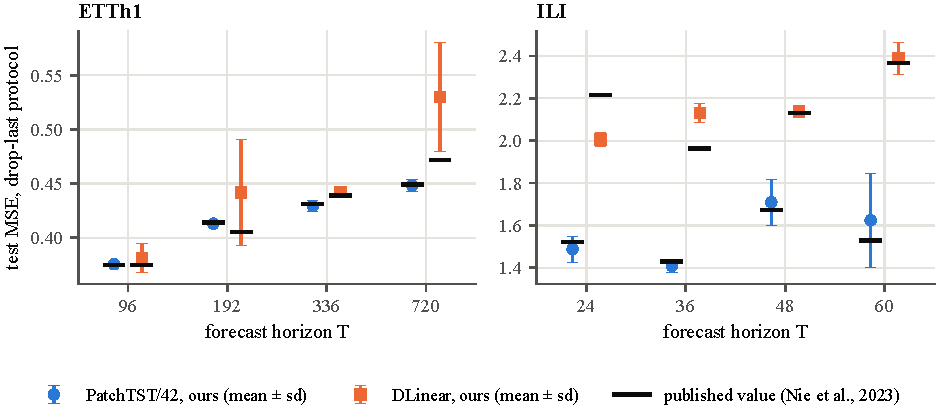
\includegraphics[width=\linewidth]{figures/fig_reproduction.pdf}
\caption{Reproduced drop-last test MSE (mean \textpm{} standard deviation over three seeds) and the published values. Horizontal bars mark the published value of the model plotted next to them.}\label{fig:1}
\end{figure}

\subsection{Four-horizon averages}
The proposal's headline metric is the error averaged over the four horizons of each benchmark (Table~\ref{tab:7}). Under the drop-last protocol, PatchTST/42 averages 0.4165 on ETTh1 and 1.5571 on ILI, against the published 0.417 and 1.539. Under the exact protocol that the proposal prescribes, it averages 0.4217 and 1.8307. These exact averages, with seed spreads of 0.0031 and 0.0693, are the reference a new design must beat by more than the spread.

\begin{table}[htbp]
\centering
\caption{Test error averaged over the four horizons, mean \textpm{} standard deviation over seeds (each seed's errors are first averaged over horizons). Published averages as in Table I of the proposal.}\label{tab:7}
{\footnotesize\setlength{\tabcolsep}{3pt}
\begin{tabular}{>{\raggedright\arraybackslash}p{\dimexpr 0.1308\linewidth-2\tabcolsep\relax}>{\raggedright\arraybackslash}p{\dimexpr 0.0846\linewidth-2\tabcolsep\relax}>{\raggedleft\arraybackslash}p{\dimexpr 0.1462\linewidth-2\tabcolsep\relax}>{\raggedleft\arraybackslash}p{\dimexpr 0.1462\linewidth-2\tabcolsep\relax}>{\raggedleft\arraybackslash}p{\dimexpr 0.1000\linewidth-2\tabcolsep\relax}>{\raggedleft\arraybackslash}p{\dimexpr 0.1462\linewidth-2\tabcolsep\relax}>{\raggedleft\arraybackslash}p{\dimexpr 0.1462\linewidth-2\tabcolsep\relax}>{\raggedleft\arraybackslash}p{\dimexpr 0.1000\linewidth-2\tabcolsep\relax}}
\toprule
\textbf{model} & \textbf{dataset} & \textbf{MSE exact} & \textbf{MSE drop-last} & \textbf{published MSE} & \textbf{MAE exact} & \textbf{MAE drop-last} & \textbf{published MAE} \\
\midrule
PatchTST/42 & ETTh1 & 0.4217 \textpm{} 0.0031 & 0.4165 \textpm{} 0.0030 & 0.417 & 0.4330 \textpm{} 0.0021 & 0.4301 \textpm{} 0.0021 & 0.431 \\
DLinear & ETTh1 & 0.4490 \textpm{} 0.0209 & 0.4488 \textpm{} 0.0210 & 0.423 & 0.4567 \textpm{} 0.0183 & 0.4564 \textpm{} 0.0184 & 0.437 \\
PatchTST/42 & ILI & 1.8307 \textpm{} 0.0693 & 1.5571 \textpm{} 0.0831 & 1.539 & 0.8821 \textpm{} 0.0221 & 0.8316 \textpm{} 0.0247 & 0.841 \\
DLinear & ILI & 2.3362 \textpm{} 0.0204 & 2.1653 \textpm{} 0.0175 & 2.169 & 1.0864 \textpm{} 0.0063 & 1.0398 \textpm{} 0.0053 & 1.041 \\
\bottomrule
\end{tabular}}
\end{table}

\subsection{Training curves}
Figure~\ref{fig:2} shows the learning curves of PatchTST/42 at the search setting and on ILI. At ETTh1 \textit{T} = 336 the validation MSE reaches its minimum at epochs 8, 9 and 17 for the three seeds and stays flat afterwards, so most of the 100 epochs bring no validation gain. Epoch 1 runs at 1/25 of the learning rate (Section 5.2), so the validation MSE after one epoch, 1.72 to 1.74, is still far from the best, 1.16 to 1.17; after epoch 2 it is 1.29 to 1.30. This matters for the referee (RQ2), whose features come from the first epoch. On ILI the validation error rises after about 15 epochs while the training loss keeps falling, a sign of overfitting on this small dataset that restoring the best validation checkpoint corrects.

\begin{figure}[htbp]
\centering
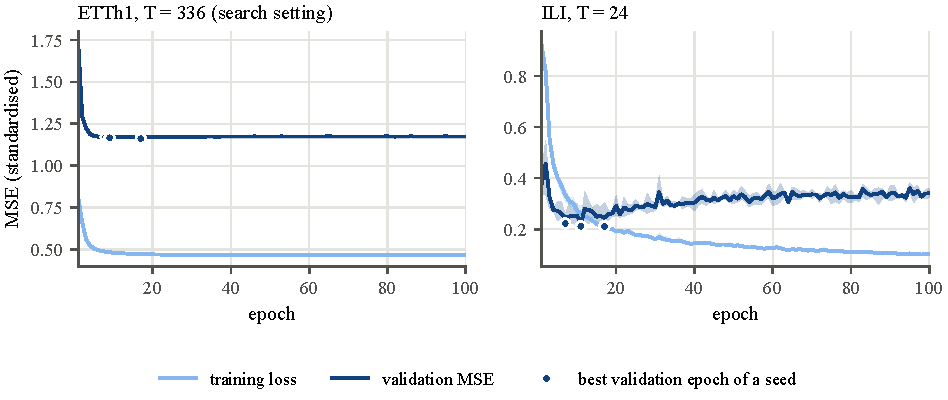
\includegraphics[width=\linewidth]{figures/fig_curves.pdf}
\caption{Training loss and validation MSE of PatchTST/42 per epoch, mean over three seeds with the range shaded. Dots mark each seed's best validation epoch, whose weights are kept.}\label{fig:2}
\end{figure}

\subsection{Sample forecasts}
Figure~\ref{fig:3} shows sample outputs of the seed-2021 models on the target variable. To avoid choosing flattering examples, each panel shows the test window whose PatchTST/42 error over all seven variables is the median of its setting. On this ETTh1 window the all-variable MSE is 0.408 for PatchTST/42 and 0.414 for DLinear; PatchTST/42 captures the daily cycle but sits below the actual oil temperature over much of the horizon, while DLinear follows the level more closely on this variable. On the ILI window the errors are 1.236 and 1.819: PatchTST/42 follows the start of the seasonal rise for about ten weeks and then turns down too early, while DLinear starts too low.

\begin{figure}[htbp]
\centering
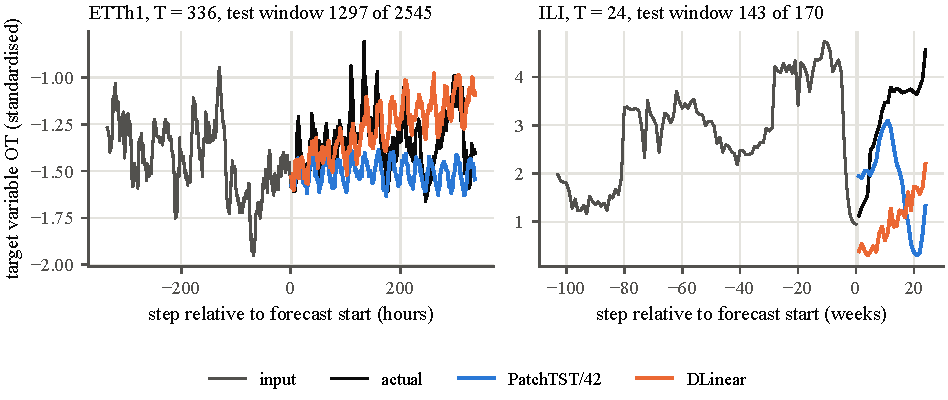
\includegraphics[width=\linewidth]{figures/fig_samples.pdf}
\caption{Sample forecasts on the target variable (OT) for the median-error test window of each setting, seed-2021 models, standardised scale. The vertical line marks the forecast start.}\label{fig:3}
\end{figure}

\subsection{PatchTST/42 against DLinear and naive forecasts}
Because both models see identical test windows, their errors can be compared window by window (Table~\ref{tab:8}, Figure~\ref{fig:4}), with a 95 percent circular block bootstrap interval (Politis and Romano, 1992) using blocks one horizon long and 2,000 resamples. PatchTST/42 has the lower mean error in all eight settings; the interval excludes zero on ETTh1 at \textit{T} = 192 and 720 and on ILI at \textit{T} = 48 and 60, while on ETTh1 at \textit{T} = 96 and 336 the two models cannot be told apart. Against two forecasts that need no training, repeating the last step and repeating the last season (one day on ETTh1, 52 weeks on ILI), PatchTST/42 is better in every setting, with error ratios of 0.68 to 0.94 against the better naive forecast; DLinear is worse than the seasonal naive forecast on ILI at \textit{T} = 36, 48 and 60 (ratios 1.01, 1.08 and 1.29).

\begin{table}[htbp]
\centering
\caption{PatchTST/42 minus DLinear, exact test MSE averaged over seeds and paired over test windows. Negative values favour PatchTST/42.}\label{tab:8}
{\footnotesize\setlength{\tabcolsep}{3pt}
\begin{tabular}{>{\raggedright\arraybackslash}p{\dimexpr 0.1500\linewidth-2\tabcolsep\relax}>{\raggedleft\arraybackslash}p{\dimexpr 0.0833\linewidth-2\tabcolsep\relax}>{\raggedleft\arraybackslash}p{\dimexpr 0.2000\linewidth-2\tabcolsep\relax}>{\raggedleft\arraybackslash}p{\dimexpr 0.2667\linewidth-2\tabcolsep\relax}>{\raggedleft\arraybackslash}p{\dimexpr 0.3000\linewidth-2\tabcolsep\relax}}
\toprule
\textbf{dataset} & \textbf{T} & \textbf{mean difference} & \textbf{95\% interval} & \textbf{windows where PatchTST/42 is better} \\
\midrule
ETTh1 & 96 & -0.0020 & -0.0107 to +0.0075 & 54\% \\
ETTh1 & 192 & -0.0288 & -0.0432 to -0.0095 & 83\% \\
ETTh1 & 336 & -0.0027 & -0.0221 to +0.0220 & 62\% \\
ETTh1 & 720 & -0.0760 & -0.1032 to -0.0518 & 98\% \\
ILI & 24 & -0.3413 & -0.8286 to +0.1882 & 81\% \\
ILI & 36 & -0.4736 & -0.9901 to +0.0190 & 89\% \\
ILI & 48 & -0.5378 & -0.9388 to -0.2182 & 83\% \\
ILI & 60 & -0.6697 & -1.0440 to -0.3315 & 92\% \\
\bottomrule
\end{tabular}}
\end{table}

\begin{figure}[htbp]
\centering
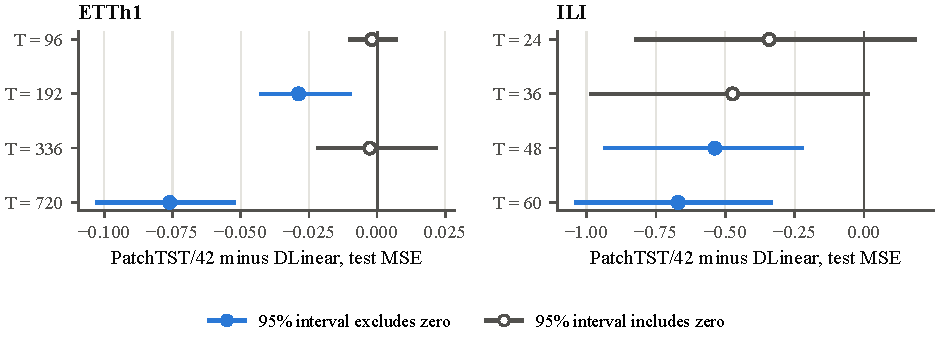
\includegraphics[width=\linewidth]{figures/fig_paired.pdf}
\caption{Paired difference in exact test MSE between PatchTST/42 and DLinear with 95 percent block-bootstrap intervals.}\label{fig:4}
\end{figure}

\subsection{Where the errors arise}
Error grows with lead time for both models (Appendix Table~\ref{tab:A2}). At the first forecast step PatchTST/42 is worse than DLinear in all eight settings (for example 0.146 against 0.103 on ETTh1 at \textit{T} = 96), while at the last step it is better in all eight (0.589 against 0.697 at step 720 of ETTh1). A plausible reading is that DLinear can weight the latest input steps directly, while PatchTST/42 reaches the horizon only through patch embeddings and a flatten head. By variable (Appendix Tables~\ref{tab:A3} and~\ref{tab:A4}), the advantage of PatchTST/42 on ETTh1 is concentrated in the oil temperature, whose error it halves at \textit{T} = 96 (0.053 against 0.107) and cuts more than fourfold at \textit{T} = 720 (0.099 against 0.436); on the six load variables the two models differ by at most 0.11 MSE. Both observations are inputs to the RQ3 analysis.

\subsection{Verification of every number}
\begin{table}[htbp]
\centering
\caption{Verification checks and their final results.}\label{tab:9}
{\footnotesize\setlength{\tabcolsep}{3pt}
\begin{tabular}{>{\raggedright\arraybackslash}p{\dimexpr 0.2083\linewidth-2\tabcolsep\relax}>{\raggedright\arraybackslash}p{\dimexpr 0.5083\linewidth-2\tabcolsep\relax}>{\raggedright\arraybackslash}p{\dimexpr 0.2833\linewidth-2\tabcolsep\relax}}
\toprule
\textbf{check} & \textbf{what it does} & \textbf{result} \\
\midrule
independent re-scoring & reloads every checkpoint and scores it on the CPU with a NumPy evaluator that shares no code with the training loop & 48 of 48 records agree; largest relative gap 1.8 \texttimes{} 10\textsuperscript{\textminus{}8} \\
archived records & the same re-scoring for the 33 superseded PatchTST records & 33 of 33 agree \\
rerun reproducibility & repeats runs with the final code and compares with first-pass records & largest difference 2.7 \texttimes{} 10\textsuperscript{\textminus{}8} over 10 runs \\
clean retraining & retrains stored DLinear runs from the command line in a fresh copy & matches records to 4 \texttimes{} 10\textsuperscript{\textminus{}10} \\
data integrity & row counts, exact columns, constant time step, finite values, split borders, window counts, parameter counts & 34 of 34 \\
leakage & multiplies every row after the training block by 1000 in a copy of the file & scaler and all training windows unchanged \\
unit tests & synthetic copies of both benchmarks plus checks on the real files & 90 of 90 pass \\
system test & copies the source without data or results, downloads data, runs tests, retrains, exercises error paths, builds and imports a wheel & 17 of 17 \\
dependency audit & pip-audit over the pinned environment & no known vulnerability in 21 packages \\
adversarial inputs & replays attacks and malformed inputs (Table~\ref{tab:14}) & 15 of 18 vulnerable, then 2 of 23, then 0 of 24 \\
\bottomrule
\end{tabular}}
\end{table}

Table~\ref{tab:9} summarises the checks. The re-scoring script rebuilds each model, loads its weights, verifies the checkpoint digest and evaluates every window with its own implementation; checkpoints trained on the Apple GPU reproduce on the CPU within 9 \texttimes{} 10\textsuperscript{\textminus{}9}. The leakage test multiplies every row after the training block by 1000 in a copy of each file, after which the fitted scaler and every training window are unchanged while the change is visible in the test windows. Because the architect will write thousands of configurations, the code was also attacked with malformed and hostile inputs; Section 5.6 and Table~\ref{tab:14} describe what was found and fixed.

\section{Challenges and Changes from the Proposal}
\subsection{The test protocol and the project target}
\textbf{Issue.} Our first exact ILI results were far above the published values (PatchTST/42 at \textit{T} = 24: 1.93 against 1.522). The official test loaders drop the last incomplete batch, and because test windows are ordered in time the dropped windows are always the most recent ones (Table~\ref{tab:10}). On ETTh1 at most 113 of more than 2,000 windows are dropped and the protocols differ by at most 0.0102 MSE, but on ILI the ten dropped windows at \textit{T} = 24 have an MSE of 9.00 against 1.49 for the 160 kept windows. Their targets run from November 2019 to June 2020, the 2019 to 2020 influenza season and the first months of the COVID-19 pandemic, and Figure~\ref{fig:5} shows the error climbing over exactly these windows. Because the kept count depends on the batch size, the drop-last test set even changes with a training hyperparameter.

\textbf{How we handled it.} Every run now records both protocols. The published values were produced with drop-last loaders in both code bases (LTSF-Linear switched to keeping every window only in March 2023, after publication), so drop-last is the like-for-like comparison, and on that protocol the reproduction matches (Section 4.2). \textbf{Change from the proposal:} the target is restated as beating our reproduced PatchTST/42 under the exact protocol (Section 2.1), because the published averages that the proposal quotes cannot be compared with the exact protocol the proposal also requires.

\begin{table}[htbp]
\centering
\caption{Windows removed by the drop-last protocol and their error (seed means). The MSE of the kept windows is the drop-last mean.}\label{tab:10}
{\footnotesize\setlength{\tabcolsep}{3pt}
\begin{tabular}{>{\raggedright\arraybackslash}p{\dimexpr 0.1610\linewidth-2\tabcolsep\relax}>{\raggedright\arraybackslash}p{\dimexpr 0.1017\linewidth-2\tabcolsep\relax}>{\raggedleft\arraybackslash}p{\dimexpr 0.0678\linewidth-2\tabcolsep\relax}>{\raggedleft\arraybackslash}p{\dimexpr 0.1186\linewidth-2\tabcolsep\relax}>{\raggedleft\arraybackslash}p{\dimexpr 0.1102\linewidth-2\tabcolsep\relax}>{\raggedleft\arraybackslash}p{\dimexpr 0.1441\linewidth-2\tabcolsep\relax}>{\raggedleft\arraybackslash}p{\dimexpr 0.1525\linewidth-2\tabcolsep\relax}>{\raggedleft\arraybackslash}p{\dimexpr 0.1441\linewidth-2\tabcolsep\relax}}
\toprule
\textbf{model} & \textbf{dataset} & \textbf{T} & \textbf{windows} & \textbf{dropped} & \textbf{MSE kept} & \textbf{MSE dropped} & \textbf{MSE exact} \\
\midrule
PatchTST/42 & ETTh1 & 96 & 2,785 & 97 & 0.3754 & 0.4821 & 0.3791 \\
PatchTST/42 & ETTh1 & 192 & 2,689 & 1 & 0.4129 & 0.5327 & 0.4130 \\
PatchTST/42 & ETTh1 & 336 & 2,545 & 113 & 0.4293 & 0.6602 & 0.4395 \\
PatchTST/42 & ETTh1 & 720 & 2,161 & 113 & 0.4483 & 0.5787 & 0.4551 \\
PatchTST/42 & ILI & 24 & 170 & 10 & 1.4867 & 9.0048 & 1.9289 \\
PatchTST/42 & ILI & 36 & 158 & 14 & 1.4086 & 6.1162 & 1.8258 \\
PatchTST/42 & ILI & 48 & 146 & 2 & 1.7090 & 6.1510 & 1.7699 \\
PatchTST/42 & ILI & 60 & 134 & 6 & 1.6239 & 5.5126 & 1.7981 \\
DLinear & ETTh1 & 96 & 2,785 & 1 & 0.3810 & 0.5223 & 0.3811 \\
DLinear & ETTh1 & 192 & 2,689 & 1 & 0.4417 & 0.5346 & 0.4417 \\
DLinear & ETTh1 & 336 & 2,545 & 17 & 0.4422 & 0.4483 & 0.4422 \\
DLinear & ETTh1 & 720 & 2,161 & 17 & 0.5301 & 0.6531 & 0.5311 \\
DLinear & ILI & 24 & 170 & 10 & 2.0054 & 6.5077 & 2.2702 \\
DLinear & ILI & 36 & 158 & 30 & 2.1312 & 3.0164 & 2.2993 \\
DLinear & ILI & 48 & 146 & 18 & 2.1368 & 3.5224 & 2.3077 \\
DLinear & ILI & 60 & 134 & 6 & 2.3877 & 4.1743 & 2.4677 \\
\bottomrule
\end{tabular}}
\end{table}

\begin{figure}[htbp]
\centering
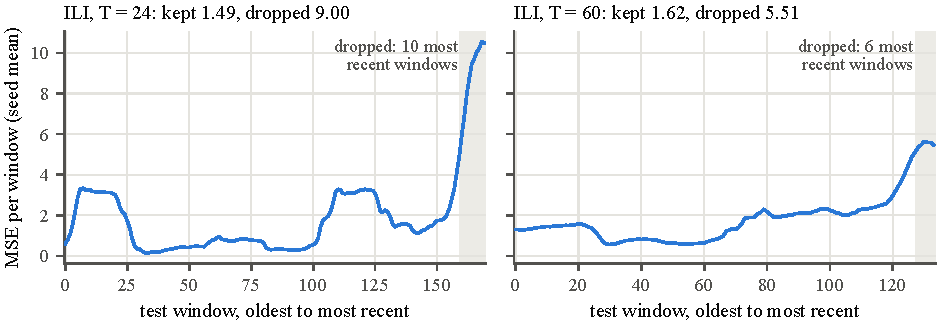
\includegraphics[width=\linewidth]{figures/fig_dropped_windows.pdf}
\caption{Test MSE of each ILI window for PatchTST/42, averaged over three seeds, from the oldest to the most recent window. The shaded region marks the windows that the drop-last loader discards.}\label{fig:5}
\end{figure}

\subsection{Training settings hidden in the official code}
\textbf{Issue.} Even with the drop-last protocol, the first ILI results were 3 to 15 percent above the published values. A line-by-line audit of the official code found two settings that do not appear among the published hyperparameters. First, the official ILI script passes a constant learning rate, while our first configuration decayed it. Second, the official PatchTST trainer constructs a OneCycleLR scheduler (Smith and Topin, 2019) for every run but advances it only for one schedule option. Construction alone changes the optimiser: the PyTorch implementation sets Adam's $\beta$\textsubscript{1} to 0.95 and the learning rate to 1/25 of its maximum. The per-epoch schedule overwrites the rate after epoch 1 but never resets $\beta$\textsubscript{1}, so every published PatchTST result was trained with $\beta$\textsubscript{1} = 0.95 and a 25-fold lower first-epoch rate.

\textbf{How we handled it.} Both settings are reproduced (Table~\ref{tab:5}), a unit test constructs the official scheduler and confirms the two values, the 33 affected records were archived, and every PatchTST run was repeated. Table~\ref{tab:11} and Figure~\ref{fig:6} trace the effect. The schedule alone changed the ILI drop-last means by less than 0.006 at \textit{T} = 24 to 48 and by +0.078 at \textit{T} = 60, within the seed spread of 0.22 there; the optimiser state lowered them by 2.7 to 7.4 percent and moved every horizon closer to the published value, while on ETTh1 it changed the means by at most 0.0017. An effect of this size, had it come from an architecture change, would have been read as a meaningful improvement, so the search will use exactly this recipe for every candidate.

\begin{table}[htbp]
\centering
\caption{Drop-last test MSE of PatchTST/42 (mean \textpm{} standard deviation over three seeds) after each correction. ETTh1 already used its official schedule; ETTh1 at \textit{T} = 720 was first run after both corrections.}\label{tab:11}
{\footnotesize\setlength{\tabcolsep}{3pt}
\begin{tabular}{>{\raggedright\arraybackslash}p{\dimexpr 0.1083\linewidth-2\tabcolsep\relax}>{\raggedleft\arraybackslash}p{\dimexpr 0.0667\linewidth-2\tabcolsep\relax}>{\raggedleft\arraybackslash}p{\dimexpr 0.1250\linewidth-2\tabcolsep\relax}>{\raggedleft\arraybackslash}p{\dimexpr 0.2250\linewidth-2\tabcolsep\relax}>{\raggedleft\arraybackslash}p{\dimexpr 0.2333\linewidth-2\tabcolsep\relax}>{\raggedleft\arraybackslash}p{\dimexpr 0.2417\linewidth-2\tabcolsep\relax}}
\toprule
\textbf{dataset} & \textbf{T} & \textbf{published} & \textbf{type3 schedule, $\beta$\textsubscript{1} 0.9} & \textbf{official schedule, $\beta$\textsubscript{1} 0.9} & \textbf{official schedule and optimiser state} \\
\midrule
ETTh1 & 96 & 0.375 & not run & 0.3737 \textpm{} 0.0004 & 0.3754 \textpm{} 0.0005 \\
ETTh1 & 192 & 0.414 & not run & 0.4118 \textpm{} 0.0017 & 0.4129 \textpm{} 0.0013 \\
ETTh1 & 336 & 0.431 & not run & 0.4298 \textpm{} 0.0041 & 0.4293 \textpm{} 0.0050 \\
ILI & 24 & 1.522 & 1.5631 \textpm{} 0.1088 & 1.5652 \textpm{} 0.1991 & 1.4867 \textpm{} 0.0614 \\
ILI & 36 & 1.430 & 1.4939 \textpm{} 0.2277 & 1.4921 \textpm{} 0.2218 & 1.4086 \textpm{} 0.0310 \\
ILI & 48 & 1.673 & 1.7513 \textpm{} 0.1457 & 1.7564 \textpm{} 0.1696 & 1.7090 \textpm{} 0.1100 \\
ILI & 60 & 1.529 & 1.6753 \textpm{} 0.2234 & 1.7529 \textpm{} 0.0415 & 1.6239 \textpm{} 0.2221 \\
\bottomrule
\end{tabular}}
\end{table}

\begin{figure}[htbp]
\centering
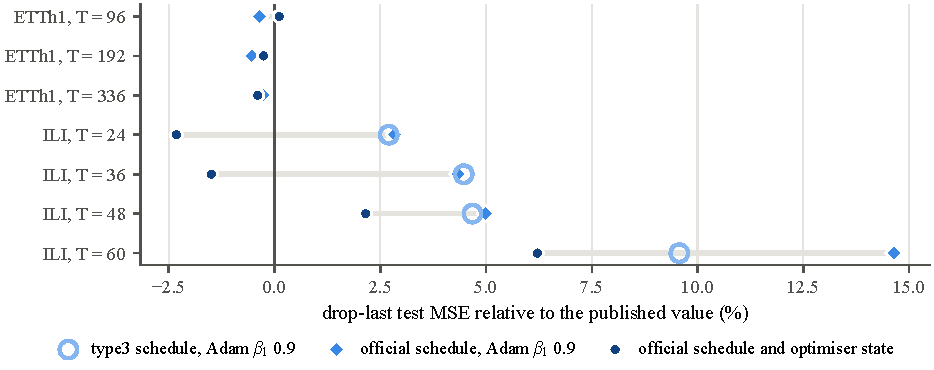
\includegraphics[width=\linewidth]{figures/fig_ablation.pdf}
\caption{Relative gap between the drop-last test MSE of PatchTST/42 and the published value after each correction. Points on the vertical line match the published value exactly.}\label{fig:6}
\end{figure}

\subsection{The parameter cap leaves a small part of the design space}
\textbf{Issue.} The proposal caps every design at the parameter count of our PatchTST/42 reproduction. Counting with the project's own model code shows how much of the grid survives the cap (Table~\ref{tab:12}). At the search setting, ETTh1 with \textit{T} = 336 and a cap of 243,248 parameters, only 2,656 of the 30,720 configurations (8.6 percent) fit. Every one of them has width 16 or 32 and treats variables independently: no configuration with width 64, 128 or 256 and no channel-mixing configuration fits. The cause is the flatten head, 93 percent of PatchTST/42's parameters at this horizon, whose size grows with the product of width and patch count, so a wider encoder must be paid for with fewer patches. Of the 2,656 feasible configurations, 2,368 also fit the cap at all eight settings.

\textbf{Changes from the proposal.} Random search and regularized evolution will sample and mutate only within the 2,368 configurations that fit at every setting, so that no trained candidate is spent on a design that would be rejected and the winner found at \textit{T} = 336 can be retrained everywhere within budget. The architect's prompt will state the cap, and proposals above it will be rejected before training. RQ3 will treat width and variable handling as constrained by the budget rather than as free choices.

\begin{table}[htbp]
\centering
\caption{Configurations of the 30,720-point grid whose parameter count does not exceed the PatchTST/42 reproduction, counted by building every configuration with the project's model code.}\label{tab:12}
{\footnotesize\setlength{\tabcolsep}{3pt}
\begin{tabular}{>{\raggedright\arraybackslash}p{\dimexpr 0.1579\linewidth-2\tabcolsep\relax}>{\raggedleft\arraybackslash}p{\dimexpr 0.0877\linewidth-2\tabcolsep\relax}>{\raggedleft\arraybackslash}p{\dimexpr 0.2281\linewidth-2\tabcolsep\relax}>{\raggedleft\arraybackslash}p{\dimexpr 0.3158\linewidth-2\tabcolsep\relax}>{\raggedleft\arraybackslash}p{\dimexpr 0.2105\linewidth-2\tabcolsep\relax}}
\toprule
\textbf{dataset} & \textbf{T} & \textbf{parameter cap} & \textbf{configurations within cap} & \textbf{share of grid} \\
\midrule
ETTh1 & 96 & 81,728 & 2,720 & 8.9\% \\
ETTh1 & 192 & 146,336 & 2,752 & 9.0\% \\
ETTh1 & 336 & 243,248 & 2,656 & 8.6\% \\
ETTh1 & 720 & 501,680 & 2,464 & 8.0\% \\
ILI & 24 & 33,400 & 6,144 & 20.0\% \\
ILI & 36 & 41,476 & 6,016 & 19.6\% \\
ILI & 48 & 49,552 & 6,048 & 19.7\% \\
ILI & 60 & 57,628 & 6,048 & 19.7\% \\
\bottomrule
\end{tabular}}
\end{table}

\subsection{A verified reimplementation instead of adapting the official code}
\textbf{Change from the proposal.} The proposal planned to adapt the official PatchTST implementation and to run DLinear from its authors' code. We instead reimplemented the data pipeline, both models, the training loop and the evaluation in one package and verified each part against the official code: configurations line by line, split borders, window counts, parameter counts equal to hand counts, and the published numbers. The nine design fields, strict validation of machine-written configurations, per-epoch logging for the referee, attention capture and both test protocols were simpler to build into one small code base than to retrofit into two. The reimplementation is also what exposed the hidden optimiser state of Section 5.2; reusing the official trainer would have carried it into every search run unnoticed. Attention maps are stored by the model during the forward pass rather than read through forward hooks, which gives the same information.

\subsection{Seed sensitivity of DLinear}
\textbf{Issue.} DLinear trains for at most ten epochs with patience 3 and a rate that halves every epoch from the third, so a run whose validation error rises for three epochs after the first stops at epoch 4 with its first-epoch weights. This happened to seed 2023 at \textit{T} = 192 (test MSE 0.498) and seed 2022 at \textit{T} = 720 (0.578). \textbf{How we handled it.} Seven more seeds were run for every DLinear setting (Table~\ref{tab:13}, Figure~\ref{fig:7}). With ten seeds the ETTh1 gaps shrink to 5.6 percent at \textit{T} = 192 and 8.5 percent at \textit{T} = 720; the published value lies inside the range of our ten seeds at \textit{T} = 96, 336 and 720, but at \textit{T} = 192 every seed is above it, the best by 0.003. The remaining gap is unexplained and is listed as an open issue.

\begin{table}[htbp]
\centering
\caption{Drop-last test MSE of DLinear on ETTh1 with three and with ten seeds.}\label{tab:13}
{\footnotesize\setlength{\tabcolsep}{3pt}
\begin{tabular}{>{\raggedleft\arraybackslash}p{\dimexpr 0.0744\linewidth-2\tabcolsep\relax}>{\raggedleft\arraybackslash}p{\dimexpr 0.1901\linewidth-2\tabcolsep\relax}>{\raggedleft\arraybackslash}p{\dimexpr 0.1901\linewidth-2\tabcolsep\relax}>{\raggedleft\arraybackslash}p{\dimexpr 0.2149\linewidth-2\tabcolsep\relax}>{\raggedleft\arraybackslash}p{\dimexpr 0.2066\linewidth-2\tabcolsep\relax}>{\raggedleft\arraybackslash}p{\dimexpr 0.1240\linewidth-2\tabcolsep\relax}}
\toprule
\textbf{T} & \textbf{3 seeds} & \textbf{10 seeds} & \textbf{range over 10 seeds} & \textbf{seeds stopped at epoch 1} & \textbf{published} \\
\midrule
96 & 0.3810 \textpm{} 0.0133 & 0.3760 \textpm{} 0.0080 & 0.3703 to 0.3962 & 0 & 0.375 \\
192 & 0.4417 \textpm{} 0.0494 & 0.4275 \textpm{} 0.0284 & 0.4081 to 0.4984 & 1 & 0.405 \\
336 & 0.4422 \textpm{} 0.0025 & 0.4443 \textpm{} 0.0069 & 0.4373 to 0.4602 & 0 & 0.439 \\
720 & 0.5301 \textpm{} 0.0502 & 0.5119 \textpm{} 0.0373 & 0.4702 to 0.5777 & 2 & 0.472 \\
\bottomrule
\end{tabular}}
\end{table}

\begin{figure}[htbp]
\centering
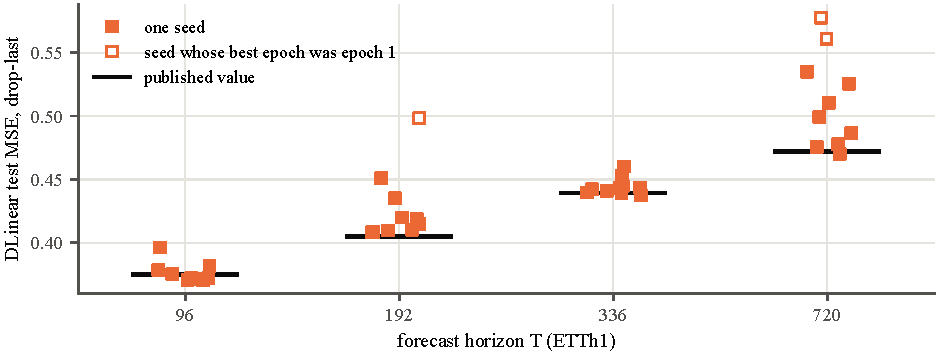
\includegraphics[width=\linewidth]{figures/fig_dlinear_seeds.pdf}
\caption{Drop-last test MSE of DLinear on ETTh1 for ten seeds per horizon. Hollow markers are runs whose best validation epoch was the first.}\label{fig:7}
\end{figure}

\subsection{Engineering issues}
\begin{itemize}
\item \textbf{GPU evaluation failure.} The first error accumulator cast to 64-bit floats on the device, which the Apple MPS backend does not support, so the first GPU run failed at its first evaluation. Errors are now summed on the device and cast on the CPU, and a test checks that GPU and CPU agree to four digits.
\item \textbf{Interrupted runs.} Long training chains stopped when the controlling session ended. Runs are now launched as detached processes, can be resumed with a skip-existing option, and a stale-record check refuses to reuse records made with other settings.
\item \textbf{Unsafe or malformed input.} The first adversarial round found 15 of 18 probes vulnerable, from a run name that escaped the output folder to a diverged run recorded as normal (Table~\ref{tab:14}). After fixes and regression tests the second round found 2 of 23 and the third none of 24.
\item \textbf{A correction to the proposal.} The proposal states that the ILI data run from 2002 to 2021; the file ends on 30 June 2020 (966 weeks).
\end{itemize}

\begin{table}[htbp]
\centering
\caption{Categories of adversarial probes, with an example, the behaviour of the original code and the fix.}\label{tab:14}
{\footnotesize\setlength{\tabcolsep}{3pt}
\begin{tabular}{>{\raggedright\arraybackslash}p{\dimexpr 0.1750\linewidth-2\tabcolsep\relax}>{\raggedright\arraybackslash}p{\dimexpr 0.2750\linewidth-2\tabcolsep\relax}>{\raggedright\arraybackslash}p{\dimexpr 0.2667\linewidth-2\tabcolsep\relax}>{\raggedright\arraybackslash}p{\dimexpr 0.2833\linewidth-2\tabcolsep\relax}}
\toprule
\textbf{category} & \textbf{example probe} & \textbf{behaviour in round 1} & \textbf{fix} \\
\midrule
path handling & run tag x/../../../escaped & wrote record and checkpoint outside the output directory & tags restricted to 64 safe characters \\
deserialisation & YAML object tag; pickled checkpoint & safe & kept safe loaders; added digest and tensor-type checks \\
type confusion & instance\_norm: "false"; patch\_len: 16.5; n\_heads: 0 & accepted, or crashed with an unrelated error & strict types and ranges for every field \\
resource exhaustion & d\_model = 2\textsuperscript{20}, about 8.8 \texttimes{} 10\textsuperscript{12} parameters & accepted & caps far above the grid \\
optimisation settings & learning rate \textminus{}1, NaN, infinity or 10\textsuperscript{30} & accepted; a diverged run was recorded as normal & finite positive values; training stops on a non-finite loss and flags the record \\
malformed data & a NaN value, shuffled rows, a missing column & trained silently & exact columns, constant time step and finite values required \\
aggregation & one run in two directories; two configurations in one row & counted twice; averaged together & duplicates and mixed configurations are errors \\
stale results & skip-existing after a configuration change & kept the stale record & stored settings must match the request \\
write integrity & interrupt during a write & truncated record left on disk & write to a temporary file, then rename \\
supply chain & forged file served as ETTh1 & accepted & https only, size cap, pinned SHA-256 \\
\bottomrule
\end{tabular}}
\end{table}

\subsection{Summary of changes}
Table~\ref{tab:15} collects the changes from the proposal described in this section, with the reason for each.

\begin{table}[htbp]
\centering
\caption{Changes from the proposal.}\label{tab:15}
{\footnotesize\setlength{\tabcolsep}{3pt}
\begin{tabular}{>{\raggedright\arraybackslash}p{\dimexpr 0.1500\linewidth-2\tabcolsep\relax}>{\raggedright\arraybackslash}p{\dimexpr 0.2667\linewidth-2\tabcolsep\relax}>{\raggedright\arraybackslash}p{\dimexpr 0.3167\linewidth-2\tabcolsep\relax}>{\raggedright\arraybackslash}p{\dimexpr 0.2667\linewidth-2\tabcolsep\relax}}
\toprule
\textbf{topic} & \textbf{proposal} & \textbf{now} & \textbf{reason} \\
\midrule
target & beat the published averages 0.417 (ETTh1) and 1.539 (ILI) & beat our reproduced PatchTST/42 under the exact protocol (0.4217 and 1.8307); drop-last reported alongside & the published values are drop-last; the proposal requires every test sample \\
code base & adapt the official PatchTST code; run DLinear from its authors' code & own reimplementation, verified against both official code bases & design fields, validation, logging and both protocols in one place; exposed a hidden setting \\
training recipe & official scripts & official scripts plus the hidden optimiser state and the constant ILI schedule & needed to match the published results \\
search space & all 30,720 configurations & the 2,368 configurations within the parameter cap at every setting & the cap rules out the rest \\
seeds & three seeds & three seeds; ten for DLinear & DLinear is sensitive to early stopping \\
attention maps & read through forward hooks & stored by the model & same information, simpler \\
ILI date range & 2002 to 2021 & 2002 to June 2020 & as in the data file \\
\bottomrule
\end{tabular}}
\end{table}

\section{Remaining Work and Timeline}
Weeks 1 to 3 of the proposal are complete. The proposal planned nine more weeks, but the final report is due on 3 December 2026, about five weeks from now, so the remaining plan is compressed while keeping its order (Table~\ref{tab:16}). The baselines that RQ1 needs and the referee come first, because the architect league depends on both.

\begin{table}[htbp]
\centering
\caption{Remaining tasks, target dates and owners.}\label{tab:16}
{\footnotesize\setlength{\tabcolsep}{3pt}
\begin{tabular}{>{\raggedright\arraybackslash}p{\dimexpr 0.1083\linewidth-2\tabcolsep\relax}>{\raggedright\arraybackslash}p{\dimexpr 0.1583\linewidth-2\tabcolsep\relax}>{\raggedright\arraybackslash}p{\dimexpr 0.5250\linewidth-2\tabcolsep\relax}>{\raggedright\arraybackslash}p{\dimexpr 0.2083\linewidth-2\tabcolsep\relax}}
\toprule
\textbf{proposal weeks} & \textbf{target date} & \textbf{task} & \textbf{owner} \\
\midrule
4 to 5 & 13 November 2026 & feasible-set sampler; random search and regularized evolution on ETTh1 at \textit{T} = 336, logging one-epoch features for every candidate & Diya Pradeep \\
5 & 13 November 2026 & referee version 1 (XGBoost and two-layer network) trained on random-search candidates; Kendall's rank correlation on held-out random candidates & Sai Anirudh Katupilla \\
5 to 6 & 17 November 2026 & architect: prompt with task, budget and design space; JSON parsed by the strict configuration validator; GRPO with TRL and LoRA, eight samples per prompt & Soumitra Chavan \\
7 & 22 November 2026 & league pool of frozen architect snapshots; full LeagueTST search (about 500 one-epoch candidates, 120 full trainings) with periodic referee audits & Soumitra Chavan and Sai Anirudh Katupilla \\
8 & 24 November 2026 & RQ1 search curves (LeagueTST against random search and evolution at equal trained candidates); RQ2 rank correlation on random and on architect proposals & all \\
8 to 9 & 25 November 2026 & final training of the best design at all horizons on both datasets with three seeds; single evaluation of the test split & Diya Pradeep \\
10 & 30 November 2026 & RQ3: analysis of design choices; attention maps of the winner against PatchTST/42 & Sai Anirudh Katupilla \\
11 & date not yet announced & presentation slides & all \\
12 & 3 December 2026 & final report & all \\
\bottomrule
\end{tabular}}
\end{table}

\subsection{Compute estimate}
A PatchTST/42-sized model at ETTh1 \textit{T} = 336 takes about 4.0 seconds per epoch on the laptop GPU. Feasible designs are no larger in parameters, so 500 one-epoch screenings need roughly 35 to 45 minutes and 120 full trainings of 100 epochs roughly 13 hours, and the final training of one design at eight settings with three seeds about 3 to 5 hours. Wider feasible designs may run slower per epoch than PatchTST/42, and the cost of the architect's generation and GRPO updates has not been measured yet.

\subsection{Risks and open issues}
\begin{itemize}
\item \textbf{Compressed schedule.} Five weeks remain instead of nine. The 13-hour full-training budget fits, but the architect's GRPO training is the least predictable step; if it is not stable by its target date, the fallback below keeps RQ1 answerable.
\item \textbf{Small margins.} ETTh1 errors differ by thousandths and ILI seed spreads reach 0.22; results use three seeds, window-level bootstrap intervals and two domains.
\item \textbf{Unstable reinforcement learning.} Fallback from the proposal: use the architect as the mutation step inside regularized evolution.
\item \textbf{Referee exploitation and warm-up epoch.} Periodic full training of random candidates audits the referee; because epoch 1 runs at a reduced rate, we will test whether first- or second-epoch features rank candidates better.
\item \textbf{Overfitting the validation split.} The test split is evaluated once, for the final models.
\item \textbf{Open:} the DLinear gaps on ETTh1 at \textit{T} = 192 and 720 are only partly explained, and only one hardware platform has been used so far.
\end{itemize}

\section{Individual Contributions}
Responsibilities follow the proposal: Diya Pradeep owns data, reproduction and baselines; Soumitra Chavan owns the architect and the GRPO league; and Sai Anirudh Katupilla owns the referee, the attention analysis and the report. Table~\ref{tab:17} lists the work completed in each area and the next tasks.

\begin{table}[htbp]
\centering
\caption{Contributions so far and next tasks by member.}\label{tab:17}
{\footnotesize\setlength{\tabcolsep}{3pt}
\begin{tabular}{>{\raggedright\arraybackslash}p{\dimexpr 0.2417\linewidth-2\tabcolsep\relax}>{\raggedright\arraybackslash}p{\dimexpr 0.4583\linewidth-2\tabcolsep\relax}>{\raggedright\arraybackslash}p{\dimexpr 0.3000\linewidth-2\tabcolsep\relax}}
\toprule
\textbf{member and role} & \textbf{work so far} & \textbf{next tasks} \\
\midrule
Diya Pradeep (data, reproduction and baselines) & data pipeline and pinned downloads; DLinear; trainer; reproduction of both baselines (48 runs) and the DLinear seed study (56 runs); protocol audit and the two corrections & feasible-set random search and regularized evolution; final training of the winning design \\
Soumitra Chavan (architect and GRPO league) & configurable forecaster with nine validated fields; strict validation that rejects malformed or oversized configurations; the human-readable design-space file that the architect prompt will quote & architect prompt and JSON interface; GRPO training with TRL and LoRA; league pool \\
Sai Anirudh Katupilla (referee, attention analysis and report) & per-epoch learning curves stored in every record; attention capture in the model; independent re-scoring and statistics; adversarial testing; this report & referee and its audits (RQ2); design-choice and attention analysis (RQ3); final report \\
\bottomrule
\end{tabular}}
\end{table}

\section*{References}
\begin{list}{}{\setlength{\leftmargin}{1.5em}\setlength{\itemindent}{-1.5em}\setlength{\itemsep}{2pt}\setlength{\parsep}{0pt}}\small
\item Bergstra, J., and Bengio, Y. (2012). Random search for hyper-parameter optimization. \textit{Journal of Machine Learning Research}, 13, 281--305.
\item Chen, A., Dohan, D. M., and So, D. R. (2023). EvoPrompting: Language models for code-level neural architecture search. In \textit{Advances in Neural Information Processing Systems (NeurIPS)}, 36.
\item Chen, T., and Guestrin, C. (2016). XGBoost: A scalable tree boosting system. In \textit{Proceedings of the 22nd ACM SIGKDD International Conference on Knowledge Discovery and Data Mining}, 785--794.
\item Domhan, T., Springenberg, J. T., and Hutter, F. (2015). Speeding up automatic hyperparameter optimization of deep neural networks by extrapolation of learning curves. In \textit{Proceedings of the 24th International Joint Conference on Artificial Intelligence (IJCAI)}, 3460--3468.
\item Harris, C. R., Millman, K. J., van der Walt, S. J., Gommers, R., Virtanen, P., Cournapeau, D., et al. (2020). Array programming with NumPy. \textit{Nature}, 585, 357--362.
\item Hu, E. J., Shen, Y., Wallis, P., Allen-Zhu, Z., Li, Y., Wang, S., Wang, L., and Chen, W. (2022). LoRA: Low-rank adaptation of large language models. In \textit{International Conference on Learning Representations (ICLR)}.
\item Hui, B., Yang, J., Cui, Z., Yang, J., Liu, D., Zhang, L., et al. (2024). Qwen2.5-Coder technical report. \textit{arXiv preprint arXiv:2409.12186}.
\item Hunter, J. D. (2007). Matplotlib: A 2D graphics environment. \textit{Computing in Science and Engineering}, 9(3), 90--95.
\item Kendall, M. G. (1938). A new measure of rank correlation. \textit{Biometrika}, 30(1/2), 81--93.
\item Kim, T., Kim, J., Tae, Y., Park, C., Choi, J.-H., and Choo, J. (2022). Reversible instance normalization for accurate time-series forecasting against distribution shift. In \textit{International Conference on Learning Representations (ICLR)}.
\item Kingma, D. P., and Ba, J. (2015). Adam: A method for stochastic optimization. In \textit{International Conference on Learning Representations (ICLR)}.
\item Li, L., and Talwalkar, A. (2020). Random search and reproducibility for neural architecture search. In \textit{Proceedings of the 35th Conference on Uncertainty in Artificial Intelligence (UAI 2019)}, PMLR 115.
\item Mangrulkar, S., Gugger, S., Debut, L., Belkada, Y., Paul, S., and Bossan, B. (2022). PEFT: State-of-the-art parameter-efficient fine-tuning methods. Software, \url{https://github.com/huggingface/peft}.
\item McKinney, W. (2010). Data structures for statistical computing in Python. In \textit{Proceedings of the 9th Python in Science Conference}, 56--61.
\item Nie, Y., Nguyen, N. H., Sinthong, P., and Kalagnanam, J. (2023). A time series is worth 64 words: Long-term forecasting with transformers. In \textit{International Conference on Learning Representations (ICLR)}.
\item Paszke, A., Gross, S., Massa, F., Lerer, A., Bradbury, J., Chanan, G., et al. (2019). PyTorch: An imperative style, high-performance deep learning library. In \textit{Advances in Neural Information Processing Systems (NeurIPS)}, 32.
\item Politis, D. N., and Romano, J. P. (1992). A circular block-resampling procedure for stationary data. In R. LePage and L. Billard (Eds.), \textit{Exploring the Limits of Bootstrap}, 263--270. Wiley.
\item Real, E., Aggarwal, A., Huang, Y., and Le, Q. V. (2019). Regularized evolution for image classifier architecture search. In \textit{Proceedings of the AAAI Conference on Artificial Intelligence}, 33, 4780--4789.
\item Shao, Z., Wang, P., Zhu, Q., Xu, R., Song, J., Bi, X., Zhang, H., Zhang, M., Li, Y. K., Wu, Y., and Guo, D. (2024). DeepSeekMath: Pushing the limits of mathematical reasoning in open language models. \textit{arXiv preprint arXiv:2402.03300}.
\item Smith, L. N., and Topin, N. (2019). Super-convergence: Very fast training of neural networks using large learning rates. In \textit{Artificial Intelligence and Machine Learning for Multi-Domain Operations Applications}, Proceedings of SPIE 11006.
\item Vaswani, A., Shazeer, N., Parmar, N., Uszkoreit, J., Jones, L., Gomez, A. N., Kaiser, \L{}., and Polosukhin, I. (2017). Attention is all you need. In \textit{Advances in Neural Information Processing Systems (NeurIPS)}, 30.
\item Vinyals, O., Babuschkin, I., Czarnecki, W. M., Mathieu, M., Dudzik, A., Chung, J., et al. (2019). Grandmaster level in StarCraft II using multi-agent reinforcement learning. \textit{Nature}, 575, 350--354.
\item von Werra, L., Belkada, Y., Tunstall, L., Beeching, E., Thrush, T., Lambert, N., and Huang, S. (2020). TRL: Transformer reinforcement learning. Software, \url{https://github.com/huggingface/trl}.
\item Wen, W., Liu, H., Chen, Y., Li, H., Bender, G., and Kindermans, P.-J. (2020). Neural predictor for neural architecture search. In \textit{European Conference on Computer Vision (ECCV)}.
\item White, C., Neiswanger, W., and Savani, Y. (2021). BANANAS: Bayesian optimization with neural architectures for neural architecture search. In \textit{Proceedings of the AAAI Conference on Artificial Intelligence}, 35, 10293--10301.
\item Wu, H., Xu, J., Wang, J., and Long, M. (2021). Autoformer: Decomposition transformers with auto-correlation for long-term series forecasting. In \textit{Advances in Neural Information Processing Systems (NeurIPS)}, 34.
\item Zeng, A., Chen, M., Zhang, L., and Xu, Q. (2023). Are transformers effective for time series forecasting? In \textit{Proceedings of the AAAI Conference on Artificial Intelligence}, 37, 11121--11128.
\item Zheng, M., Su, X., You, S., Wang, F., Qian, C., Xu, C., and Albanie, S. (2023). Can GPT-4 perform neural architecture search? \textit{arXiv preprint arXiv:2304.10970}.
\item Zhou, H., Zhang, S., Peng, J., Zhang, S., Li, J., Xiong, H., and Zhang, W. (2021). Informer: Beyond efficient transformer for long sequence time-series forecasting. In \textit{Proceedings of the AAAI Conference on Artificial Intelligence}, 35, 11106--11115.
\item Zhou, T., Ma, Z., Wen, Q., Wang, X., Sun, L., and Jin, R. (2022). FEDformer: Frequency enhanced decomposed transformer for long-term series forecasting. In \textit{Proceedings of the 39th International Conference on Machine Learning (ICML)}, PMLR 162.
\end{list}

\subsection*{Datasets}
\begin{list}{}{\setlength{\leftmargin}{1.5em}\setlength{\itemindent}{-1.5em}\setlength{\itemsep}{2pt}\setlength{\parsep}{0pt}}\small
\item ETTh1. Electricity Transformer Temperature dataset, hourly subset, released with Zhou et al. (2021). \url{https://github.com/zhouhaoyi/ETDataset} (file ETT-small/ETTh1.csv).
\item ILI. United States Centers for Disease Control and Prevention, ILINet national influenza-like-illness surveillance data, \url{https://gis.cdc.gov/grasp/fluview/fluportaldashboard.html}, in the weekly copy compiled for Autoformer (Wu et al., 2021) and mirrored at \url{https://huggingface.co/datasets/thuml/Time-Series-Library} (file illness/national\_illness.csv).
\end{list}

\subsection*{Code}
\begin{list}{}{\setlength{\leftmargin}{1.5em}\setlength{\itemindent}{-1.5em}\setlength{\itemsep}{2pt}\setlength{\parsep}{0pt}}\small
\item Official PatchTST implementation (Nie et al., 2023), Apache-2.0 licence. \url{https://github.com/yuqinie98/PatchTST}.
\item Official LTSF-Linear implementation including DLinear (Zeng et al., 2023). \url{https://github.com/cure-lab/LTSF-Linear}.
\item Autoformer implementation and dataset collection (Wu et al., 2021). \url{https://github.com/thuml/Autoformer}.
\end{list}

\clearpage
\appendix
\setcounter{table}{0}
\renewcommand{\thetable}{A\arabic{table}}

\section{Detailed Results}
\begingroup\scriptsize\setlength{\tabcolsep}{3pt}
\begin{longtable}{>{\raggedright\arraybackslash}p{\dimexpr 0.1298\linewidth-2\tabcolsep\relax}>{\raggedright\arraybackslash}p{\dimexpr 0.0832\linewidth-2\tabcolsep\relax}>{\raggedleft\arraybackslash}p{\dimexpr 0.0549\linewidth-2\tabcolsep\relax}>{\raggedleft\arraybackslash}p{\dimexpr 0.0666\linewidth-2\tabcolsep\relax}>{\raggedright\arraybackslash}p{\dimexpr 0.0749\linewidth-2\tabcolsep\relax}>{\raggedleft\arraybackslash}p{\dimexpr 0.1131\linewidth-2\tabcolsep\relax}>{\raggedleft\arraybackslash}p{\dimexpr 0.0799\linewidth-2\tabcolsep\relax}>{\raggedleft\arraybackslash}p{\dimexpr 0.0915\linewidth-2\tabcolsep\relax}>{\raggedleft\arraybackslash}p{\dimexpr 0.1032\linewidth-2\tabcolsep\relax}>{\raggedleft\arraybackslash}p{\dimexpr 0.1032\linewidth-2\tabcolsep\relax}>{\raggedleft\arraybackslash}p{\dimexpr 0.0998\linewidth-2\tabcolsep\relax}}
\caption{All 48 runs. Training time is the wall-clock time of the training loop; runs on ETTh1 at \textit{T} = 96 shared the machine with CPU jobs.}\label{tab:A1} \\
\toprule
\textbf{model} & \textbf{dataset} & \textbf{T} & \textbf{seed} & \textbf{device} & \textbf{best / run epochs} & \textbf{train s} & \textbf{val MSE} & \textbf{test MSE exact} & \textbf{test MSE drop-last} & \textbf{test MAE exact} \\
\midrule
\endfirsthead
\toprule
\textbf{model} & \textbf{dataset} & \textbf{T} & \textbf{seed} & \textbf{device} & \textbf{best / run epochs} & \textbf{train s} & \textbf{val MSE} & \textbf{test MSE exact} & \textbf{test MSE drop-last} & \textbf{test MAE exact} \\
\midrule
\endhead
PatchTST/42 & ETTh1 & 96 & 2021 & MPS & 68 / 100 & 1091 & 0.6793 & 0.3791 & 0.3753 & 0.4005 \\
PatchTST/42 & ETTh1 & 96 & 2022 & MPS & 75 / 100 & 723 & 0.6757 & 0.3798 & 0.3760 & 0.4014 \\
PatchTST/42 & ETTh1 & 96 & 2023 & MPS & 81 / 100 & 526 & 0.6767 & 0.3785 & 0.3749 & 0.4009 \\
PatchTST/42 & ETTh1 & 192 & 2021 & MPS & 89 / 100 & 530 & 0.9257 & 0.4139 & 0.4139 & 0.4210 \\
PatchTST/42 & ETTh1 & 192 & 2022 & MPS & 26 / 100 & 496 & 0.9210 & 0.4136 & 0.4135 & 0.4208 \\
PatchTST/42 & ETTh1 & 192 & 2023 & MPS & 94 / 100 & 414 & 0.9225 & 0.4114 & 0.4114 & 0.4198 \\
PatchTST/42 & ETTh1 & 336 & 2021 & MPS & 8 / 100 & 383 & 1.1705 & 0.4441 & 0.4336 & 0.4433 \\
PatchTST/42 & ETTh1 & 336 & 2022 & MPS & 9 / 100 & 398 & 1.1660 & 0.4410 & 0.4303 & 0.4414 \\
PatchTST/42 & ETTh1 & 336 & 2023 & MPS & 17 / 100 & 408 & 1.1618 & 0.4336 & 0.4239 & 0.4353 \\
PatchTST/42 & ETTh1 & 720 & 2021 & MPS & 6 / 100 & 366 & 1.4512 & 0.4594 & 0.4527 & 0.4729 \\
PatchTST/42 & ETTh1 & 720 & 2022 & MPS & 5 / 100 & 366 & 1.4488 & 0.4566 & 0.4496 & 0.4720 \\
PatchTST/42 & ETTh1 & 720 & 2023 & MPS & 7 / 100 & 375 & 1.4362 & 0.4493 & 0.4425 & 0.4661 \\
PatchTST/42 & ILI & 24 & 2021 & CPU & 11 / 100 & 691 & 0.2111 & 1.9004 & 1.4681 & 0.8667 \\
PatchTST/42 & ILI & 24 & 2022 & CPU & 7 / 100 & 692 & 0.2225 & 1.9617 & 1.5552 & 0.9120 \\
PatchTST/42 & ILI & 24 & 2023 & CPU & 17 / 100 & 691 & 0.2110 & 1.9247 & 1.4367 & 0.8830 \\
PatchTST/42 & ILI & 36 & 2021 & CPU & 11 / 100 & 552 & 0.1911 & 1.8330 & 1.4291 & 0.8676 \\
PatchTST/42 & ILI & 36 & 2022 & CPU & 12 / 100 & 551 & 0.2096 & 1.9046 & 1.4238 & 0.9123 \\
PatchTST/42 & ILI & 36 & 2023 & CPU & 12 / 100 & 551 & 0.2139 & 1.7396 & 1.3730 & 0.8557 \\
PatchTST/42 & ILI & 48 & 2021 & CPU & 5 / 100 & 218 & 0.2145 & 1.8257 & 1.7705 & 0.8936 \\
PatchTST/42 & ILI & 48 & 2022 & CPU & 13 / 100 & 218 & 0.2135 & 1.8308 & 1.7746 & 0.9006 \\
PatchTST/42 & ILI & 48 & 2023 & CPU & 12 / 100 & 217 & 0.1938 & 1.6531 & 1.5820 & 0.8209 \\
PatchTST/42 & ILI & 60 & 2021 & CPU & 4 / 100 & 360 & 0.2502 & 2.0174 & 1.8804 & 0.9471 \\
PatchTST/42 & ILI & 60 & 2022 & CPU & 63 / 100 & 359 & 0.2216 & 1.6675 & 1.4986 & 0.8587 \\
PatchTST/42 & ILI & 60 & 2023 & CPU & 11 / 100 & 360 & 0.2303 & 1.7094 & 1.4928 & 0.8666 \\
DLinear & ETTh1 & 96 & 2021 & CPU & 8 / 10 & 5.0 & 0.6489 & 0.3716 & 0.3715 & 0.3934 \\
DLinear & ETTh1 & 96 & 2022 & CPU & 6 / 9 & 3.4 & 0.6402 & 0.3755 & 0.3754 & 0.3986 \\
DLinear & ETTh1 & 96 & 2023 & CPU & 4 / 7 & 2.5 & 0.6383 & 0.3963 & 0.3962 & 0.4231 \\
DLinear & ETTh1 & 192 & 2021 & CPU & 5 / 8 & 10 & 0.8559 & 0.4186 & 0.4186 & 0.4284 \\
DLinear & ETTh1 & 192 & 2022 & CPU & 6 / 9 & 11 & 0.8646 & 0.4081 & 0.4081 & 0.4176 \\
DLinear & ETTh1 & 192 & 2023 & CPU & 1 / 4 & 5.9 & 0.8715 & 0.4984 & 0.4984 & 0.4965 \\
DLinear & ETTh1 & 336 & 2021 & CPU & 6 / 9 & 15 & 1.0530 & 0.4398 & 0.4397 & 0.4407 \\
DLinear & ETTh1 & 336 & 2022 & CPU & 7 / 10 & 16 & 1.0452 & 0.4421 & 0.4421 & 0.4443 \\
DLinear & ETTh1 & 336 & 2023 & CPU & 5 / 8 & 12 & 1.0403 & 0.4448 & 0.4447 & 0.4473 \\
DLinear & ETTh1 & 720 & 2021 & CPU & 6 / 9 & 20 & 1.2105 & 0.4786 & 0.4776 & 0.4926 \\
DLinear & ETTh1 & 720 & 2022 & CPU & 1 / 4 & 8.7 & 1.2572 & 0.5788 & 0.5777 & 0.5626 \\
DLinear & ETTh1 & 720 & 2023 & CPU & 3 / 6 & 13 & 1.2204 & 0.5360 & 0.5351 & 0.5350 \\
DLinear & ILI & 24 & 2021 & CPU & 3 / 6 & 0.5 & 0.2715 & 2.3306 & 2.0438 & 1.0908 \\
DLinear & ILI & 24 & 2022 & CPU & 6 / 9 & 0.7 & 0.2915 & 2.2392 & 1.9765 & 1.0402 \\
DLinear & ILI & 24 & 2023 & CPU & 7 / 10 & 0.8 & 0.2893 & 2.2410 & 1.9959 & 1.0441 \\
DLinear & ILI & 36 & 2021 & CPU & 4 / 7 & 0.5 & 0.2566 & 2.2512 & 2.0796 & 1.0576 \\
DLinear & ILI & 36 & 2022 & CPU & 4 / 7 & 0.5 & 0.2579 & 2.3324 & 2.1681 & 1.0858 \\
DLinear & ILI & 36 & 2023 & CPU & 3 / 6 & 0.4 & 0.2599 & 2.3143 & 2.1460 & 1.0875 \\
DLinear & ILI & 48 & 2021 & CPU & 3 / 6 & 0.3 & 0.2303 & 2.3620 & 2.1388 & 1.1013 \\
DLinear & ILI & 48 & 2022 & CPU & 5 / 8 & 0.4 & 0.2454 & 2.2703 & 2.1256 & 1.0722 \\
DLinear & ILI & 48 & 2023 & CPU & 6 / 9 & 0.5 & 0.2503 & 2.2907 & 2.1461 & 1.0773 \\
DLinear & ILI & 60 & 2021 & CPU & 5 / 8 & 0.5 & 0.2630 & 2.4520 & 2.3707 & 1.1211 \\
DLinear & ILI & 60 & 2022 & CPU & 3 / 6 & 0.3 & 0.2652 & 2.5463 & 2.4707 & 1.1469 \\
DLinear & ILI & 60 & 2023 & CPU & 5 / 8 & 0.4 & 0.2572 & 2.4049 & 2.3218 & 1.1114 \\
\bottomrule
\end{longtable}
\endgroup

\begin{table}[htbp]
\centering
\caption{Error by forecast step (seed mean).}\label{tab:A2}
{\footnotesize\setlength{\tabcolsep}{3pt}
\begin{tabular}{>{\raggedright\arraybackslash}p{\dimexpr 0.1583\linewidth-2\tabcolsep\relax}>{\raggedright\arraybackslash}p{\dimexpr 0.1000\linewidth-2\tabcolsep\relax}>{\raggedleft\arraybackslash}p{\dimexpr 0.0667\linewidth-2\tabcolsep\relax}>{\raggedright\arraybackslash}p{\dimexpr 0.2333\linewidth-2\tabcolsep\relax}>{\raggedright\arraybackslash}p{\dimexpr 0.4417\linewidth-2\tabcolsep\relax}}
\toprule
\textbf{model} & \textbf{dataset} & \textbf{T} & \textbf{forecast steps} & \textbf{exact test MSE at those steps} \\
\midrule
PatchTST/42 & ETTh1 & 96 & 1, 24, 48, 72, 96 & 0.1462, 0.3283, 0.3577, 0.3883, 0.4162 \\
PatchTST/42 & ETTh1 & 192 & 1, 48, 96, 144, 192 & 0.1509, 0.3527, 0.4162, 0.4452, 0.4581 \\
PatchTST/42 & ETTh1 & 336 & 1, 84, 168, 252, 336 & 0.1894, 0.4284, 0.4476, 0.4739, 0.4634 \\
PatchTST/42 & ETTh1 & 720 & 1, 180, 360, 540, 720 & 0.2260, 0.4397, 0.4232, 0.4891, 0.5892 \\
PatchTST/42 & ILI & 24 & 1, 6, 12, 18, 24 & 0.4501, 1.3366, 1.7532, 2.5872, 3.1044 \\
PatchTST/42 & ILI & 36 & 1, 9, 18, 27, 36 & 0.5851, 1.4467, 1.5104, 2.4043, 2.9366 \\
PatchTST/42 & ILI & 48 & 1, 12, 24, 36, 48 & 0.6566, 1.5386, 1.5894, 1.7804, 3.1961 \\
PatchTST/42 & ILI & 60 & 1, 15, 30, 45, 60 & 0.5058, 1.7135, 1.4026, 1.7254, 3.4644 \\
DLinear & ETTh1 & 96 & 1, 24, 48, 72, 96 & 0.1032, 0.3279, 0.3689, 0.4093, 0.4225 \\
DLinear & ETTh1 & 192 & 1, 48, 96, 144, 192 & 0.1146, 0.3633, 0.4295, 0.4808, 0.4902 \\
DLinear & ETTh1 & 336 & 1, 84, 168, 252, 336 & 0.1073, 0.4169, 0.4510, 0.4853, 0.4875 \\
DLinear & ETTh1 & 720 & 1, 180, 360, 540, 720 & 0.1168, 0.4563, 0.4841, 0.6191, 0.6965 \\
DLinear & ILI & 24 & 1, 6, 12, 18, 24 & 0.2410, 1.5111, 2.4335, 2.9569, 3.3055 \\
DLinear & ILI & 36 & 1, 9, 18, 27, 36 & 0.3088, 2.1114, 2.4874, 2.8098, 3.1080 \\
DLinear & ILI & 48 & 1, 12, 24, 36, 48 & 0.3068, 2.5265, 2.4115, 2.1448, 3.2101 \\
DLinear & ILI & 60 & 1, 15, 30, 45, 60 & 0.2386, 2.9331, 2.2364, 2.4187, 3.8216 \\
\bottomrule
\end{tabular}}
\end{table}

\begin{table}[htbp]
\centering
\caption{Error by variable on ETTh1 (exact test MSE, seed mean).}\label{tab:A3}
{\scriptsize\setlength{\tabcolsep}{3pt}
\begin{tabular}{>{\raggedright\arraybackslash}p{\dimexpr 0.1431\linewidth-2\tabcolsep\relax}>{\raggedleft\arraybackslash}p{\dimexpr 0.0673\linewidth-2\tabcolsep\relax}>{\raggedleft\arraybackslash}p{\dimexpr 0.1128\linewidth-2\tabcolsep\relax}>{\raggedleft\arraybackslash}p{\dimexpr 0.1128\linewidth-2\tabcolsep\relax}>{\raggedleft\arraybackslash}p{\dimexpr 0.1128\linewidth-2\tabcolsep\relax}>{\raggedleft\arraybackslash}p{\dimexpr 0.1128\linewidth-2\tabcolsep\relax}>{\raggedleft\arraybackslash}p{\dimexpr 0.1128\linewidth-2\tabcolsep\relax}>{\raggedleft\arraybackslash}p{\dimexpr 0.1128\linewidth-2\tabcolsep\relax}>{\raggedleft\arraybackslash}p{\dimexpr 0.1128\linewidth-2\tabcolsep\relax}}
\toprule
\textbf{model} & \textbf{T} & \textbf{HUFL} & \textbf{HULL} & \textbf{MUFL} & \textbf{MULL} & \textbf{LUFL} & \textbf{LULL} & \textbf{OT} \\
\midrule
PatchTST/42 & 96 & 0.784 & 0.212 & 0.806 & 0.172 & 0.508 & 0.119 & 0.053 \\
PatchTST/42 & 192 & 0.855 & 0.235 & 0.877 & 0.188 & 0.536 & 0.131 & 0.068 \\
PatchTST/42 & 336 & 0.905 & 0.247 & 0.919 & 0.197 & 0.583 & 0.147 & 0.079 \\
PatchTST/42 & 720 & 0.881 & 0.255 & 0.873 & 0.204 & 0.697 & 0.176 & 0.099 \\
DLinear & 96 & 0.755 & 0.213 & 0.780 & 0.173 & 0.516 & 0.124 & 0.107 \\
DLinear & 192 & 0.857 & 0.254 & 0.884 & 0.203 & 0.569 & 0.144 & 0.182 \\
DLinear & 336 & 0.854 & 0.254 & 0.871 & 0.202 & 0.596 & 0.149 & 0.170 \\
DLinear & 720 & 0.861 & 0.324 & 0.854 & 0.255 & 0.800 & 0.187 & 0.436 \\
\bottomrule
\end{tabular}}
\end{table}

\begin{table}[htbp]
\centering
\caption{Error by variable on ILI (exact test MSE, seed mean).}\label{tab:A4}
{\scriptsize\setlength{\tabcolsep}{3pt}
\begin{tabular}{>{\raggedright\arraybackslash}p{\dimexpr 0.1431\linewidth-2\tabcolsep\relax}>{\raggedleft\arraybackslash}p{\dimexpr 0.0673\linewidth-2\tabcolsep\relax}>{\raggedleft\arraybackslash}p{\dimexpr 0.1128\linewidth-2\tabcolsep\relax}>{\raggedleft\arraybackslash}p{\dimexpr 0.1128\linewidth-2\tabcolsep\relax}>{\raggedleft\arraybackslash}p{\dimexpr 0.1128\linewidth-2\tabcolsep\relax}>{\raggedleft\arraybackslash}p{\dimexpr 0.1128\linewidth-2\tabcolsep\relax}>{\raggedleft\arraybackslash}p{\dimexpr 0.1128\linewidth-2\tabcolsep\relax}>{\raggedleft\arraybackslash}p{\dimexpr 0.1128\linewidth-2\tabcolsep\relax}>{\raggedleft\arraybackslash}p{\dimexpr 0.1128\linewidth-2\tabcolsep\relax}}
\toprule
\textbf{model} & \textbf{T} & \textbf{weighted ILI \%} & \textbf{unweighted ILI \%} & \textbf{age 0-4} & \textbf{age 5-24} & \textbf{ILI total} & \textbf{providers} & \textbf{OT} \\
\midrule
PatchTST/42 & 24 & 0.924 & 1.207 & 3.213 & 2.761 & 3.889 & 0.428 & 1.080 \\
PatchTST/42 & 36 & 0.792 & 1.058 & 3.003 & 2.726 & 3.631 & 0.531 & 1.038 \\
PatchTST/42 & 48 & 0.754 & 1.028 & 2.908 & 2.705 & 3.564 & 0.542 & 0.888 \\
PatchTST/42 & 60 & 0.709 & 0.973 & 2.807 & 2.884 & 3.636 & 0.623 & 0.953 \\
DLinear & 24 & 0.941 & 1.222 & 3.420 & 2.941 & 4.234 & 1.323 & 1.810 \\
DLinear & 36 & 0.838 & 1.114 & 3.320 & 2.825 & 4.266 & 1.583 & 2.149 \\
DLinear & 48 & 0.788 & 1.064 & 3.392 & 2.770 & 4.304 & 1.620 & 2.217 \\
DLinear & 60 & 0.785 & 1.066 & 3.538 & 2.893 & 4.655 & 1.813 & 2.523 \\
\bottomrule
\end{tabular}}
\end{table}

\end{document}
